\documentclass[12pt]{article}

\usepackage{graphicx}
\usepackage{indentfirst} % garante que a primeira linha terá identação.
\usepackage{listings}
\usepackage{xcolor}
\usepackage{hyperref}       % Permite o uso de hyperlinks no texto, com um link clicável

\definecolor{codegreen}{rgb}{0,0.6,0}
\definecolor{codegray}{rgb}{0.5,0.5,0.5}
\definecolor{codepurple}{rgb}{0.58,0,0.82}
\definecolor{backcolour}{rgb}{0.95,0.95,0.92}

\lstdefinestyle{mystyle}{
    backgroundcolor=\color{backcolour},   
    commentstyle=\color{codegreen},
    keywordstyle=\color{magenta},
    numberstyle=\tiny\color{codegray},
    stringstyle=\color{codepurple},
    basicstyle=\ttfamily\footnotesize,
    breakatwhitespace=false,         
    breaklines=true,                 
    captionpos=b,                    
    keepspaces=true,                 
    numbers=left,                    
    numbersep=5pt,                  
    showspaces=false,                
    showstringspaces=false,
    showtabs=false,                  
    tabsize=2
}

\lstset{style=mystyle}
\newcommand{\blue}[1]{\textcolor{blue}{#1}}

\title{API Segura com Autenticação de Mensagens}
\author{Gabriel Henrique do Nascimento Neres \\ Arthur Diehl Barroso}
\date{\today}

\begin{document}
\maketitle

\begin{abstract}
  Texto detalhando o desenvolvimento de uma versão simplificada do algoritmo de criptografia DES, denominado de S-DES, que realiza a encriptação e decriptação utilizando dois modos de operação, o ECB e CBC. Nele é utilizado uma chave de 10 bits e uma entrada de convertida em uma lista de bytes. 

  \textbf{Palavras-chave}: Criptografia, DES, ECB, CBC.
\end{abstract}

Nesse trabalho foi proposto o desenvolvimento de uma API que utilizasse do conteúdo visto ao longo da disciplina para garantir alguma forma de segurança nas requisições feitas a API. Para a realização desse trabalho, foi utilizada a linguagem de programação Java com o framework Quarkus e o auxílio de bibliotecas para a realização das requisições.

\section{API Rest}
Para dar início no desenvolvimento do trabalho, é preciso desenvolver uma aplicação que possua as características mínimas de uma API baseado no sistema REST. As principais características levadas em consideração para o desenvolvimento da API REST simbólica para o trabalho foram:

\begin{itemize}
  \item Ser Stateless, ou seja, cada requisição deve ter todas as informações necessárias para o tratamento da requisição;
  \item Fazer uso dos métodos HTTP (GEt, POSt, PUT, \dots);
  \item Ser baseada em recursos, sendo organizada por funções que são identificadas por URLs únicas.
\end{itemize}

Baseado nessas características o módulo \textbf{Servidor} da API foi desenvolvido, possuindo 2 endpoints, um para requisições GET e outro para requisições POST. O método GET foi definido para ser acessado por meio do caminho \blue{server/get/\{body\}}, no qual o parâmetro \blue{body} representa a informação necessária para a consulta ao servidor, enquanto o método POST é acessado pelo caminho \blue{server/post} que deverá receber um corpo na requisição HTTP para a obtenção dos dados necessário para o servidor. o Código implementado está na imagem \ref{fig:Endpoints}

\begin{figure}[h]
    \centering
    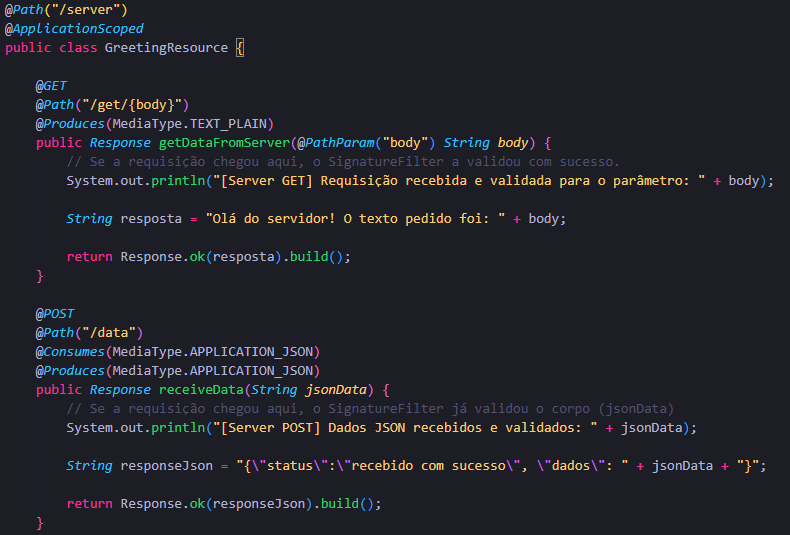
\includegraphics[width = 0.8\linewidth]{Imagens/Endpoints.png}  
    \label{fig:Endpoints}
\end{figure}

Para o desenvolvimento da parte responsável por realizar a segurança da API, foi adicionada a classe \textbf{SignatureFilter} que será responsável por substituir o filtro padrão utilizado pela aplicação pela versão personalizada que será desenvolvida.

Na parte do cliente que será responsável por acessar a API do servidor, foi desenvolvido o módulo \textbf{Cliente} que também possui 2 endpoints, se enquadrando como uma API REST se deixada separada, dedicado a interagir com uma tela HTML. Essa abordagem foi escolhida para simplificar a realização dos testes e deixar a visualização mais amigável para o usuário, e assim criando um sistema composto por requisições feitas a um servidor a partir de uma aplicação web, composta pela tela (HTML) e o seu backend (cliente). No módulo cliente também foram inseridos as funcionalidades ligadas a etapa de segurança do trabalho. 

\section{Camada de segurança}
O processo de segurança escolhido para a aplicação foi o de fornecer autenticidade as requisições trocadas do cliente ao servidor. Nesse contexto, foi utilizado um sistema baseado em certificado digital, o qual é utilizado para assinar as mensagens a serem enviadas e por meio da chave pública verificar a autenticidade da assinatura. 

Para iniciar o processo, precisamos criar um certificado para ser utilizado nas nossas requisições. Nesse sentido, foi utilizada a própria JWT do java com a keystore para gerar um certificado autoassinado, que para os propósitos de teste teriam todos os recursos necessário, embora não transmita credibilidade em situações reais de utilização de algum sistema, precisando algum terceiro certificar esse certificado. Para a realização dos acessos aos dados de certificado do usuário foi criada a classe \textbf{CryptoUtils} (\ref{fig:CryptoUtils}) que recebe as credenciais de acesso ao certificado e retorna a aplicação o certificado e a chave privada. 

\begin{figure}[h]
    \centering
    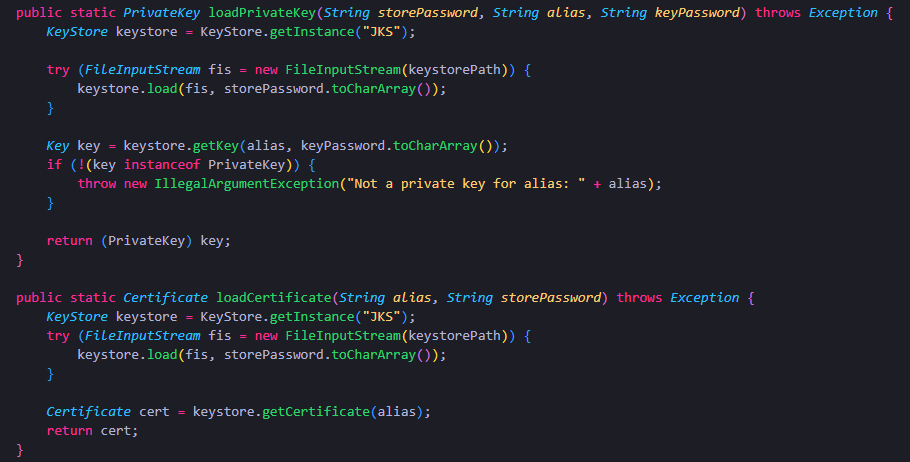
\includegraphics[width = 0.8\linewidth]{Imagens/CryptoUtils.png}  
    \label{fig:CryptoUtils}
\end{figure}

No processo de garantia da autenticidade da mensagem a ser encaminhada ao servidor, o corpo da mensagem a ser enviada é transformada em um \textbf{hash} por meio do algoritmo SHA-256 e é assinado utilizando o RSA, ou seja, criptografa o hash obtido da etapa anterior utilizando a chave privada do usuário, podendo ser revertida a mensagem original com a chave pública e por esse motivo não garante confidenciabilidade nesse processo. 


\subsection{GET}
Para a requisição do tipo GET, a qual não possui um corpo de requisição, foi preciso

\subsection{POST}
Nas requisições feitas por meio do post, o próprio corpo da mensagem foi utilizado para a assinatura, sem a inclusão de elementos adicionais;


\section{Problemas observados}
Durante a implementação alguns problemas de segurança foram observados no protótipo final obtido. Os principais problemas observados foram:
\begin{itemize}
  \item A cada requisição é preciso obter os dados do certificado para a realização de assinatura da mensagem, deixando o processo muito mais lento;
  \item Falta de meios para as credenciais do usuário serem passadas a aplicação (cliente), sendo uma falha para a segurança do processo;
  \item Falta de confidenciabilidade da mensagem enviada;
\end{itemize}

Dentre as soluções para os problemas encontrados estão:
\begin{itemize}
  \item Utilização de tokens nas requisições;
  \item Ao transferir a autenticidade para outro meio (token), a confidenciabilidade do processo pode ser melhorada de maneira mais simples;
\end{itemize}



% \begin{lstlisting}[language=Python]
% def permutation(s: str, indices: list[int]) -> str:
%     return ''.join(s[i] for i in indices)
% \end{lstlisting}

\section{Código}
O código está disponível no github pelo link: \href{https://github.com/TheMasterGame0/Rest-Seguro}{https://github.com/TheMasterGame0/Rest-Seguro}

\end{document}